% add your introduction section here ...
``\textit{This includes an example of an opening quote, the inclusion and reference to a Figure and a (chapter-specific) citation.}''\\
\hspace*{.83\textwidth}{\citepim{Darwin1859}} %note the section-specific citation commands (indication section and within text (i/a/b/c/z), and self reference from the chapter title (p/m))

\begin{multicols}{2}
\section{First Section}

\begin{figure*}[!hb] % figure will be placed after the next paragraph finishes
\centering
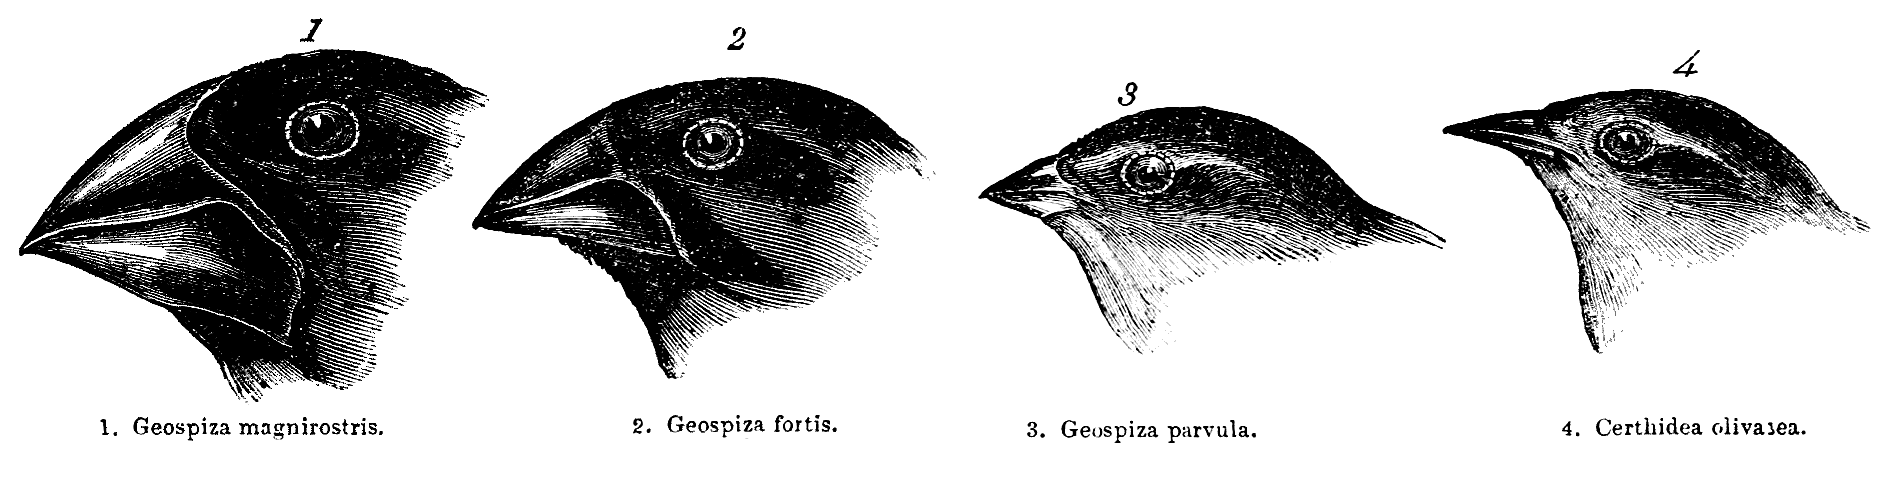
\includegraphics[width = \fwidth]{figures/ci/finches.png}
\caption[Darwins Finches]{\label{fig:cif1}\textbf{Darwins Finches.} These are such famous birds.
}
\end{figure*}

Here is some demonstration how to reference a Figure (using the label from the figure command) --- just look at these birds (\figref{fig:cif1}).
The reference is done using the command \textsw{$\backslash figref\{\}$}.
The rest is just dummy text....

\lipsum[1-4]

\section{Second Section}

\lipsum[5-6]

\bibliographystyleim{apalikeK}
\bibliographyim{library/ci.bib}
\end{multicols}
